\documentclass[
../../AuD-Zusammenfassung.tex,
]
{subfiles}

\externaldocument[ext:]{../../AuD-Zusammenfassung}
% Set Graphics Path, so pictures load correctly
\graphicspath{{../../}}

\begin{document}
\section{Advanced Design}
\subsection{Divide \& Conquer}
\subsubsection{Fourier-Transformation}
Das Allgemeine Konzept der Fourier-Transformation ist die Lösung eines Problems, welches in ungünstiger Form vorliegt. Demnach wird das Problem erst in eine geeignetere Darstellung umgewandelt, diese dann bearbeitet und anschließend zurückgewandelt. Dies kann im Endeffekt schneller sein als das Problem in der ungünstigen Form zu bearbeiten. Als Beispiel wird im folgenden die Polynommultiplikation verwendet.\\
Polynome liegen normalerweise in der Koeffizientendarstellung vor:
\begin{center}
    $p(x) = p_0 + p_1x + p_2x^2 + \ldots + p_{n-2}x^{n-2} + p_{n-1}x^{n-1}$\\
    mit $p_{n-1} \not= 0$ und grad(p(x)) = $n - 1$
\end{center}
Wenn so ein Polynom beispielsweise als Array der Koeffizienten gegeben ist, so kann man ein Polynom an der Stelle $x = w$ einfach mit dem folgenden Algorithmus ausrechnen:\\
\begin{algorithm}[H]
    \SetKwFunction{poly}{polyEval}
    \tcp{Complexity: $\Theta(n)$}
    \tcp{p: Array of coefficients, w: evaluation point(x)}
    \Fn{\poly{p, w}}{
        n = length(p)\;
        result = p[n-1]; \tcp{Initializes result to last (biggest) coefficient}
        \tcp{Runs from last to first coefficient, excluding the last one as its already in result}
        \For{i = n - 2 \KwDownTo 0}{
            result = result * w + p[i]; \tcp{Because of the loop each coefficient gets multiplied as often as it needs to}
        }
        \KwRet{result}\;
    }
\end{algorithm}
So ergibt sich essenziell:
\begin{center}
    $p(x) = (((p_{n-1}x + p_{n-2})x + p_{n-3})\ldots p_1)x + p_0$
\end{center}
Als konkretes Beispiel kann man zum Beispiel das Polynom $p(x) = 2 + 3x + 5x^2$ und w = 2 nehmen. Das Array würde dementsprechend dann so aussehen: p[] = [2, 3, 5].
So würde die letzendliche Rechenoperation so aussehen:
\begin{center}
    $p(2) = (5 \cdot 2 + 3) \cdot 2 + 2 = 28$ 
\end{center}
\newpage
Das Multiplizieren zweier Polynome ist allerdings schon komplexer. So wäre die Multiplikation zweier Polynome vom Grad n-1 formell: 
\begin{center}
    $p(x) \cdot q(x) = (\sum_{i=0}^{n-1}p_ix^i) \cdot (\sum_{i=0}^{n-1}q_ix^i)$ = $\sum_{k=0}^{2n-2}(\sum_{j=0}^{k}p_j\cdot q_{k-j})x^k$\\
    Vom Grad 2n-2
\end{center}
Dies kann mit dem folgenden Algorithmus dargestellt werden:\\
\begin{algorithm}[H]
    \SetKwFunction{poly}{polyMult}
    \tcp{Complexity: $\Theta(n^2)$}
    \tcp{p: Array of coefficients, q: Array of coefficients}
    \Fn{\poly{p, q}}{
        n = length(p)\;
        result = new Array(2n - 1); \tcp{Initializes result to new Array of length 2n - 1}
        \tcp{For all coefficients that are gonna be in the result}
        \For{k = 0 \KwTo 2n - 2}{
            result[k] = 0; \tcp{Initializes result[k] to 0}
            \tcp{For all coefficients smaller-equal the current one}
            \For{j = 0 \KwTo k}{
                result[k] = result[k] + p[j] * q[k - j]; \tcp{Multiplies current result with the corresponding coefficients at j in p and k-j in q}
            }
        }
        \KwRet{result}\;
    }
\end{algorithm}
Dies ist aber mit $\Theta(n^2)$ relativ langsam. Mithilfe der Fourier-Transformation kann man die Rechenzeit auf $\Theta(n \log n)$ reduzieren, indem man die Koeffizientendarstellung in Punkt/Wert Darstellung umwandelt. 
Das Allgemeine Schema sieht dann also so aus:\\

\begin{figure}[htp]
    \centering
    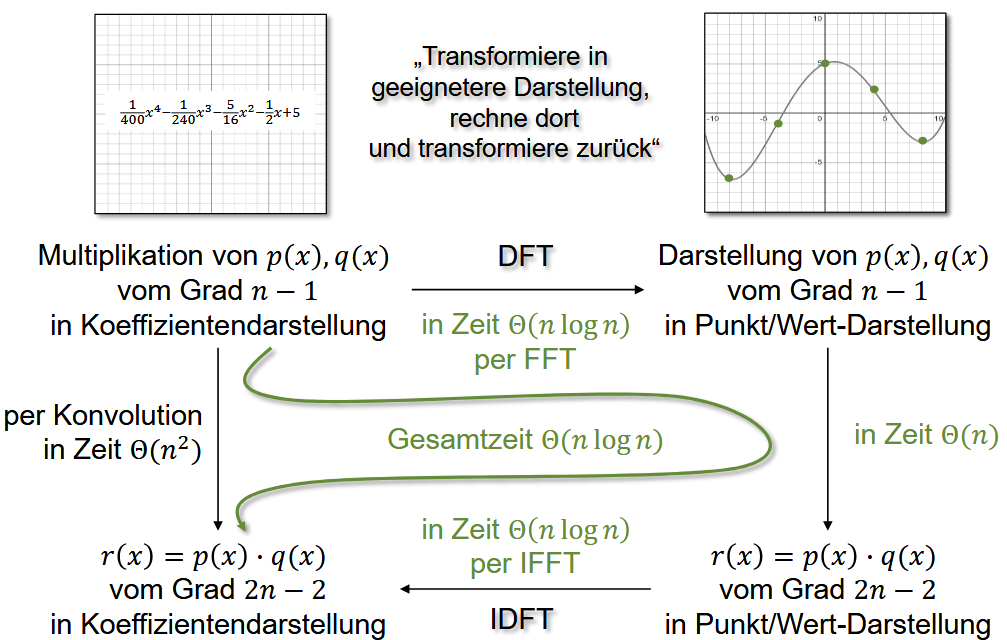
\includegraphics[scale = 0.6]{Pics/FourierTransPolySchema.png}
\end{figure}
Die Punkt/Wert Darstellung eines Polynoms kann auch wieder über ein Array dargestellt werden, bei dem jeder Eintrag p[i] p[i].x und p[i].y besitzt. \\
So kann man in dieser Form das Produkt $r(x) = p(x) \cdot q(x)$ leicht in $\Theta(n)$ ausrechnen, indem man für jede x-Koordinate $x_j$ in $j = 0, 1, \ldots, 2n -1$ $r(x_j) = p(x_j) \cdot q(x_j)$ ausrechnet. Die x Koordinate korrespondiert dann mit dem Grad des Koeffizienten.\\
\begin{algorithm}[H]
    \SetKwFunction{poly}{polyMult}
    \tcp{Complexity: $\Theta(n)$}
    \tcp{p: Array of coefficients, q: Array of coefficients}
    \Fn{\poly{p, q}}{
        n = length(p)\;
        result = new Array(2n - 1); \tcp{Initializes result to new Array of length 2n - 1}
        \tcp{For all coefficients that are gonna be in the result}
        \For{i = 0 \KwTo 2n - 2}{
            result[i].x = p[i].x; \tcp{x stays the same}
            result[i].y = p[i].y * q[i].y; \tcp{y of the result is the product of y of p and y of q}
        }
        \KwRet{result}\;
    }
\end{algorithm}

Nun brauchen wir nur noch die Umwandlung von Koeffizientendarstellung in Punkt/Wert Darstellung und vice versa. Diese wird in der Fourier Transformation als \textit{Discrete Fourier-Transform} und \textit{Inverse Discrete Fourier-Transform} bezeichnet.\\
Die Fourier-Transformation bei Polynomen geht nach dem folgenden Schema:\\
\begin{enumerate}
    \item Schreibe p(x) in Form $p(x) = p_{even}(x^2) + x\cdot P_{odd}(x^2)$ mit $p_{even}(x) = p_0 + p_2x + \ldots + p_{n-2}x^{(n-2)/2}$ und $p_{odd}(x) = p_1 + p_3x + \ldots + p_{n-1}x^{(n-2)/2}$ \\
    $p_{even}$ und $p_{odd}$ sind nun jeweils Polynome von ca. halben Grad.
    \item Nun können wir Werte $x_j$ nutzen, so dass $x_j^2 = x_{j+n}^2$ für alle $j = 0, 1, \ldots, n - 1$ und $x_j \not= x_{j+n}$.\\
    Somit müssen $p_{odd}$ und $p_{even}$ vom Grad $\frac{n-2}{2} = \frac{n}{2} - 1$ nur an n Stellen $x_0^2, x_1^2, \ldots, x_{n-1}^2$ gewertet werten. Demnach ist die Problemgröße halbiert und das Divide and Conquer Prinzip kann angewendet werden.
\end{enumerate}

\begin{algorithm}[H]
    \SetKwFunction{poly}{polyFFT}
    \tcp{Complexity: $\Theta(n \log n)$}
    \tcp{p: Array of coefficients, w: unit root (starts at 2n)}
    \Fn{\poly{p, w}}{
        n = length(p)\;
        $p_{even}$ = new Array(n/2); $p_{odd}$ = new Array(n/2); \tcp{Initializes $p_{even}$ and $p_{odd}$ to new Arrays of length n/2}
        pVal = new Array(2n); $p_{even}$Val = new Array(n); $p_{odd}$Val = new Array(n); \tcp{Initializes pVal and $p_{even}$Val and $p_{odd}$Val to new Arrays of length 2n and n respectively}
        x = new Array(2n); x[0] = 1;\tcp{Initializes x to new Array of length 2n, holds the x values of the coefficient}
        \For{i = 1 \KwTo 2n-1}{
            x[i] = w * x[i - 1]; \tcp{Essentially does x[i] = $w^i$}
        }
        \tcp{If the polynomial is constant, only needs to assign first and second coefficient. Base-Case.}
        \If{n == 1}{
            pVal[0].x = x[0]; pVal[0].y = p[0].y; \tcp{Assigns first coefficient.x the corresponding value from x[] and the corresponding value from the polynomial}
        } \Else{

            \tcp{Fills $p_{even}$ and $p_{odd}$ with the values from p}
            \For{i = 0 \KwTo (n-2)/2}{
                $p_{even}$[i] = p[2i]; $p_{odd}$[i] = p[2i + 1]\; 
            }
            \tcp{Recursively call polyFFT on $p_{even}$ and $p_{odd}$}
            $p_{even}$Val = \poly{$p_{even}$, w*w}; \tcp{Evaluates at $x_j^2$} 
            $p_{odd}$Val = \poly{$p_{odd}$, w*w}\; 
            \tcp{Essentially calculates $p(x_j) = p_{even}(x_j^2) + x_j \cdot p_{odd}(x_j^2)$ for all elements in pVal}
            \For{i = 0 \KwTo 2n-1}{
                pVal[i].x = x[i]; \tcp{Assigns coefficient.x the corresponding value from x[]}
                pVal[i].y = $p_{even}$Val[i \% n] + x[i] * $p_{odd}$Val[i \% n].y\;
            }
        }
        \KwRet{pVal}\;
    }
\end{algorithm}
Die Punkt/Wert Darstellung kann prinzipiell wie folgt dargestellt werden, wo x die Polynome für jedes $x_j$ beinhaltet, p die Koeffizenten und y die Werte. Dabei werden in dem Ergebnis des Algorithmus die Koeffizienten ausgelassen.
\[\begin{pmatrix}
    1 & x_0 & \ldots & x_0^{n-1} \\
    1 & x_1 & \ldots & x_1^{n-1} \\
    \vdots & \vdots & \ddots & \vdots \\
    1 & x_{n-1} & \ldots & x_{n-1}^{n-1} 
\end{pmatrix}
\begin{pmatrix}
    p_0 \\
    p_1 \\
    \vdots \\
    p_{n-1}
\end{pmatrix}
=
\begin{pmatrix}
    y_0 \\
    y_1 \\
    \vdots \\
    y_{n-1}
\end{pmatrix}
\]\\
Nun muss noch der letzte Schritt der Fourier Transformation auf Polynommultiplikation angewendet werden, die Rückwandlung in die ursprüngliche Form (Koeffizientendarstellung). So gilt für die Koeffizienten p:\\
\[
\begin{pmatrix}
    p_0 \\
    p_1 \\
    \vdots \\
    p_{n-1}
\end{pmatrix}
=
\begin{pmatrix}
    1 & x_0 & \ldots & x_0^{n-1} \\
    1 & x_1 & \ldots & x_1^{n-1} \\
    \vdots & \vdots & \ddots & \vdots \\
    1 & x_{n-1} & \ldots & x_{n-1}^{n-1} 
\end{pmatrix}^{-1}
\cdot 
\begin{pmatrix}
    y_0 \\
    y_1 \\
    \vdots \\
    y_{n-1}
\end{pmatrix}
\]\\
Dies bedeutet also, dass wir um von der Punkt/Wert Darstellung in die Koeffizientendarstellung umzuwandeln lediglich die Inverse der Punkte mit den Werten multiplizieren müssen.

\begin{algorithm}
    \SetKwFunction{pointkey}{pointKeyIFFT}
    \SetKwFunction{iwrap}{IFFTWrapper}
    \tcp{p: Array of coefficients, Wrapper for IFFT for initial call, also renorms the result}
    \Fn{\iwrap{p}}{
        result = \pointkey{p, w}; \tcp{w starts at n}
        \For{i = 0 \KwTo n-1}{
            result[i] = result[i] / n; \tcp{Result of DFT is normed, the coefficients however are not, therefore we have to divide the result of IFFT by n}
        }
        \KwRet{result}\;
    }
    \tcp{Complexity: $\Theta(n \log n)$}
    \tcp{p: Array of coefficients, w: unit root (starts at n)}
    \Fn{\pointkey{p, w}}{
        n = length(p)\;
        result = new Array(n); result$_{even}$Val = new Array(n); result${_odd}$Val = new Array(n); \tcp{Initializes result and its values to new Array of length n}
        x = new Array(n); x[0] = 1;\tcp{Initializes x to new Array of length n, holds the x values of the coefficient}
        \For{i = 1 \KwTo n-1}{
            x[i] = w * x[i - 1]; \tcp{Essentially does x[i] = $w^i$}
        }
        \tcp{If the polynomial is constant only needs to finds first coefficient. Base-Case}
        \If{n == 1}{
            result[0] = p[0].y\;
        }
        \Else {
            result$_{even}$ = new Array(n/2); result$_{odd}$ = new Array(n/2); \tcp{Initializes result$_{even}$ and result$_{odd}$ to new Arrays of length n/2}
            \tcp{Fill result$_{even}$ with their corresponding values from p}
            \For{i = 0 \KwTo (n-2)/2 }{
                result$_{even}$Val[i] = p[2i]; result$_{odd}$Val[i] = p[2i + 1]\;
            }
            result$_{even}$ = \pointkey{result$_{even}$Val, w*w}; \tcp{Evaluates at $x_j^2$} 
            result$_{odd}$ = \pointkey{result$_{odd}$Val, w*w}\;
            \For{i = 0 \KwTo n-1}{
                result[i] = result$_{even}$[i \% n] + result$_{odd}$[i \% n] /  x[i]\;
            }
        }
        \KwRet{result}\;
    }
\end{algorithm}
\includepdf[pages={16-21}, pagecommand={},nup=2x3, frame=true, scale=0.9]{./VL Folien/07AdvancedDesigns.pdf}
\includepdf[pages={26-33}, pagecommand={},nup=2x4, frame=true, scale=0.95]{./VL Folien/07AdvancedDesigns.pdf}

\subsection{Backtracking}


\newpage
\subsection{Dynamic Programming}


\newpage
\subsection{Greedy Algorithms}

\end{document}